\section{White box lumped model for a building: RC networks}

The objective of the house model for this project is to serve as test environment for a heating model, which means that the house model is intended as a tool to enable taking building installation design decisions. The house heating demand calculation model implemented for this project is a white box \emph{lumped} model. Specifically, it is a RC network model consisting of thermal resistances (R) and capacities (C). The RC network model is based on the analogy with electrical circuits. The simulation of thermodynamic systems characterizing building elements as resistances or capacities allows to simplify the model while maintaining a high simulation results accuracy \textbf{(Bagheri et al.\cite{en11040890}, Bacher et al\cite{Bacher}.)}.  

\subsection{White box lumped models}

There are several types of RC models, the most common being 3R4C models and 3R2C models which are applied on the outer and internal building walls. For the simulation of simple house buildings 3R2C models perform as accurate as more complex 3R4C models \textbf{(Fraisse et al.\cite{Fraisse})}. Considering that one of the objectives for this project is to obtain a fast but accurate simulation of a simple dwelling the 3R2C network model appeared a good starting point. In the 3R2C model two indoor temperature nodes are present in the dwelling. with capacities (usually an air and a wall temperature) and a well-known outdoor temperature. Between these 3 temperature nodes 3 heat transfer resistances are present. However, the direct heat transfer between the inner walls and the outdoor air is low. Moreover, uncertainties are present about heat transfer coefficients between walls and indoor air, different indoor temperatures in the house rooms and the ground temperature which deviates from the outdoor temperature. In addition, occupancy behaviour varies strongly. For that reason, we have made a further simplification to a 2R2C model. In section 4 it is shown that this dwelling model delivers a reliable annual energy consumption.


\subsection{House Model R and C Values}

This section presents the basic information for calculating a house model based on an RC network. This category of house models, analogous to electrical impedance networks, may have different numbers of R and C components and may have various component topologies. For the specific model properties, references will be given.

In heat transfer theory the basic thermal circuit contains thermal resistances. Heat transfer occurs via conduction, convection and radiation. In analogy with Ohm's Law for electricity, expressions can be derived for the heat transfer rate (analogous to electrical current) and the thermal resistances (analogous to ohmic resistances) in these three modes of heat transfer. The temperature difference plays a role analogous to the electrical voltage difference. These expressions are shown in Fig.\ref{fig:lumped_table}.
\begin{figure}[H]
	\centering
	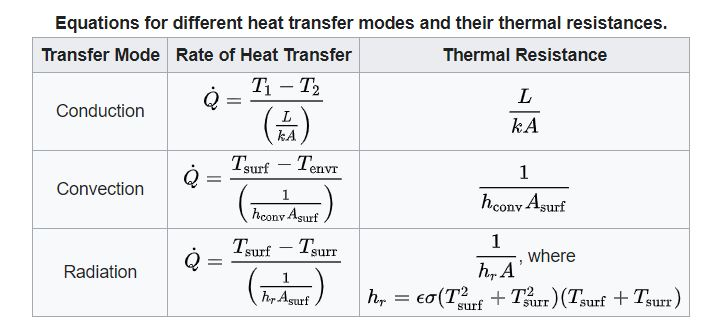
\includegraphics[width=0.6\columnwidth]{Pictures/heat transfer mode.JPG}
	\caption[Short title]{Heat transfer modes \cite{GIGO}.}
	\label{fig:lumped_table}
\end{figure}
\newpage

In \cite{HTTHERMO} and \cite{FUND} the expressions in Fig.\ref{fig:lumped_table} are derived.
For conduction, the expression for absolute thermal resistance is:  

\begin{equation}
	R = \frac{L}{kA} \qquad \left[ \frac{K}{W} \right]
\end{equation}

\begin{itemize}
    \item $L$ is the distance over which heat transfer takes place, or the thickness of the material $[m]$.
    \item $k$ (also denoted with $\lambda$) is the thermal conductivity of the material. [$\dfrac{W}{mK}$]. 
    \item $A$ is the conductive surface area  $[m^2]$.
    \item Thermal resistivity is the reciprocal of thermal conductivity and can be expressed as $r =\dfrac{1}{k}$  in $[\dfrac{mK}{W}]$

\end{itemize}

For convection and radiation the expression for thermal resistance is: $R = \dfrac{1}{h \cdot A}$ [$\dfrac{K}{W}$].

\begin{itemize}
    \item $A$ is the surface area where the heat transfer takes place $[m^2]$.
    \item $h$ is the heat transfer coefficient  [$\dfrac{W}{m^2K}$]
\end{itemize}


The $R$-value (in Dutch: $R$-waarde or $R_d$-waarde) of a building material \cite{Rvalues_insulation} is the thermal resistance of a square meter surface.
It can be calculated by multiplying the thermal \emph{resistivity} with the thickness of the material in  $m$.
Alternatively it is calculated by dividing the material thickness by the thermal \emph{conductivity} $k$ or $\lambda$.

\begin{equation}
	\text{R-value} = r \cdot L  \qquad \text{or} \qquad  \text{R-value} = \frac{L}{k}  \qquad \text{or} \qquad  
	\text{R-value} = \frac{L}{\lambda}  \qquad \left[m \cdot \frac{m \cdot K}{W} \right] = \left[\frac{m^2 \cdot K}{W}\right] 
\end{equation}


Some typical heat transfer $R$-values are: \cite{OVERALL}: 

\begin{itemize}
	\item Static layer of air, 40 mm thickness (1.57 in)  : R = 0.18 [$\frac{m^2K}{W}$].
	\item Inside heat transfer resistance, horizontal current : R = 0.13 [$\frac{m^2K}{W}$]. 
	\item Outside heat transfer resistance, horizontal current : R = 0.04 [$\frac{m^2K}{W}$].
	\item Inside heat transfer resistance, heat current from down upwards : R = 0.10 [$\frac{m^2K}{W}$].
	\item Outside heat transfer resistance, heat current from above downwards : R = 0.17 [$\frac{m^2K}{W}$].
\end{itemize}


\textbf{Note}: in Dutch building physics, $R$-values with subscripts are used:
\begin{itemize}
	\item $R_d$-waarde is used for the $R$-value of a homogeneous building material. $ R = \frac{L}{\lambda} $
	\item $R_c$-waarde (compound, construction) is used for the $R$-value of a surface consisting of several building materials. $R_c$-waarden are calculated as the surface-area weighted sum of $R_d$-waarden of the building materials. 
	For the simplest roof surface, $R_c$ is a linear combination of the $R$-values of the wooden joists and girders (spanten en gordingen) and the areas in between, filled with a certain insulation material sandwich.
	The $R$-value of the insulation sandwich, in its turn, is the sum of the $R$-values of the materials in the sandwich. From inside out, this sandwich may consist of \textit{e.g.} a 9.5 mm plaster board, a PIR/PUR insulation panel, an air gap and a wooden roof deck. All types of $R$-value have the dimension $ [\frac{m^2 \cdot K}{W}] $.
\end{itemize}

\begin{figure}[H]
	\centering
	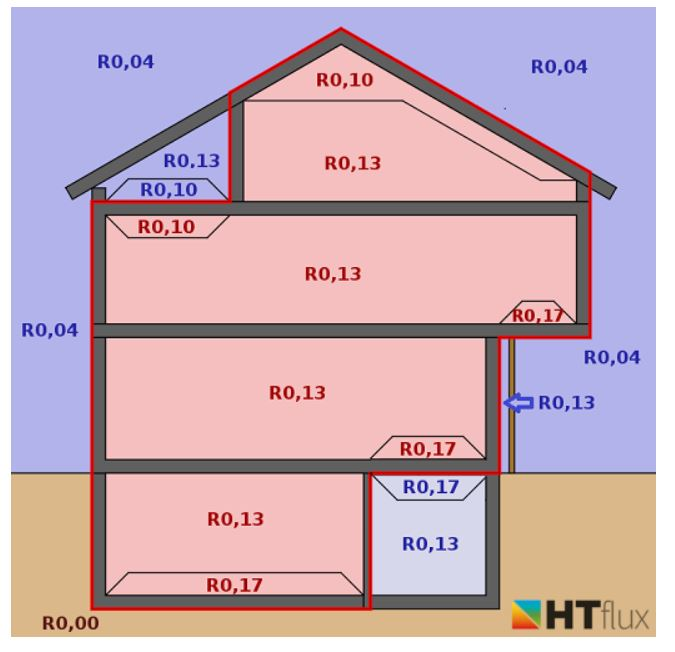
\includegraphics[width=0.6\columnwidth]{Pictures/Overview of heat resistances.JPG}
	\caption[Short title]{An overview of $R$-values for heat transfer \cite{SURFREST}.}
	\label{fig:overview}
\end{figure}


The standard R\textsubscript{c}-values that have been used for facades, roof and floor until 2020 are summarized in Fig.\ref{fig:Rcvalues}:

\begin{figure}[H]
	\centering
	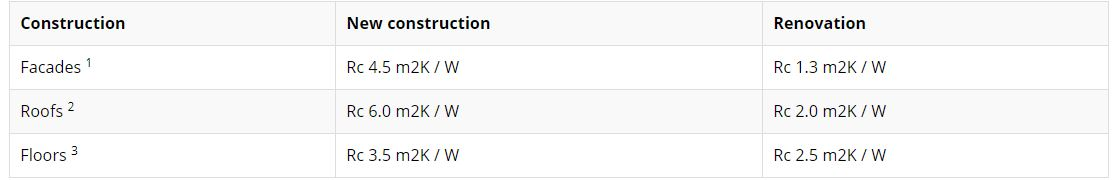
\includegraphics[width=1.0\columnwidth]{Pictures/Rc_values_2020.JPG}
	\caption[Short title]{R\textsubscript{c} Values \cite{ISOL}}
	\label{fig:Rcvalues}
\end{figure}

New standard values will be used from 1-1-2021, since the building standard NEN 1068 will be replaced by the NTA 8800 standard. The old and new situation is described in "EnergieVademecum Energiebewust ontwerpen van nieuwbouwwoningen", Hoofdstuk 5: Thermische isolatie, thermische bruggen en luchtdichtheid.
\cite{ISSO}.

\begin{figure}[H]
	\centering
	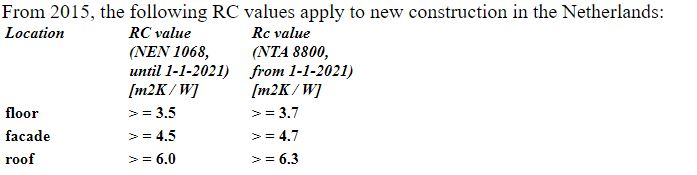
\includegraphics[width=0.8\columnwidth]{Pictures/Rc_values_2021.JPG}
	\caption[Short title]{R\textsubscript{c} Values \cite{RVALUE}}
	\label{fig:newRc}
\end{figure}

The values used for different types of houses such as: row houses, detached houses and apartments can be found in the document "Voorbeeldwoningen 2011" \cite{VOORBEELD}. An example with values for a common type of row house, built in the period from 1975 to 1991 is shown in Fig. \ref{row_house}:


\begin{figure}[H]
	\centering
	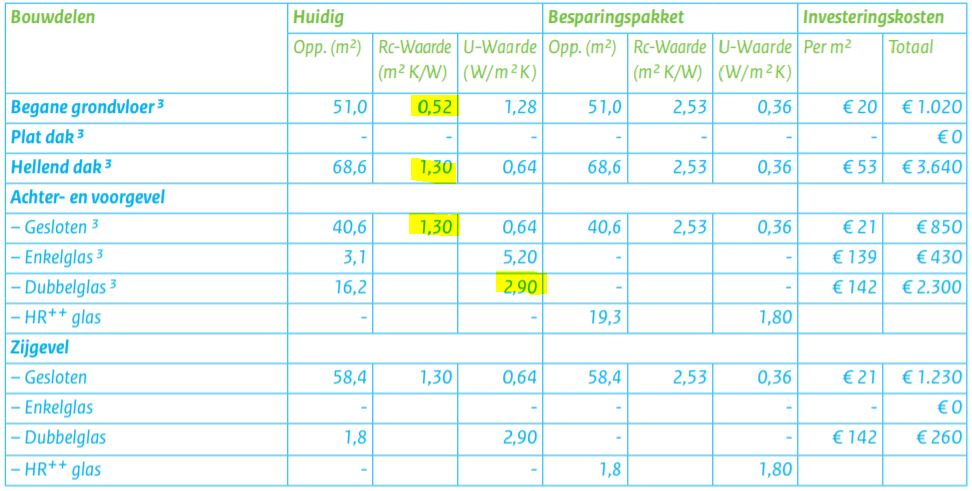
\includegraphics[width=0.8\columnwidth]{Pictures/row_house_1975-1991.JPG}
	\caption[Short title]{R\textsubscript{c}-values for a row house type built between 1975-1991 \cite{VOORBEELD}}
	\label{row_house}
\end{figure} 

\subsection{Thermal building (envelope) model analogous to a 2R-2C electrical network}

The heat transfer in a building will be modelled in analogy to an electrical circuit where \emph{heat transfer rate} is analogous to by current, \emph{temperature} difference is analogous to potential difference, heat sources are represented by constant current sources, absolute thermal resistances are represented by resistors and thermal capacity ()heat capacity) by capacitors \cite{AbsTR}. Figure \ref{fig:Analogies} summarizes the similar term use in different fields.

\begin{figure}[H]
	\centering
	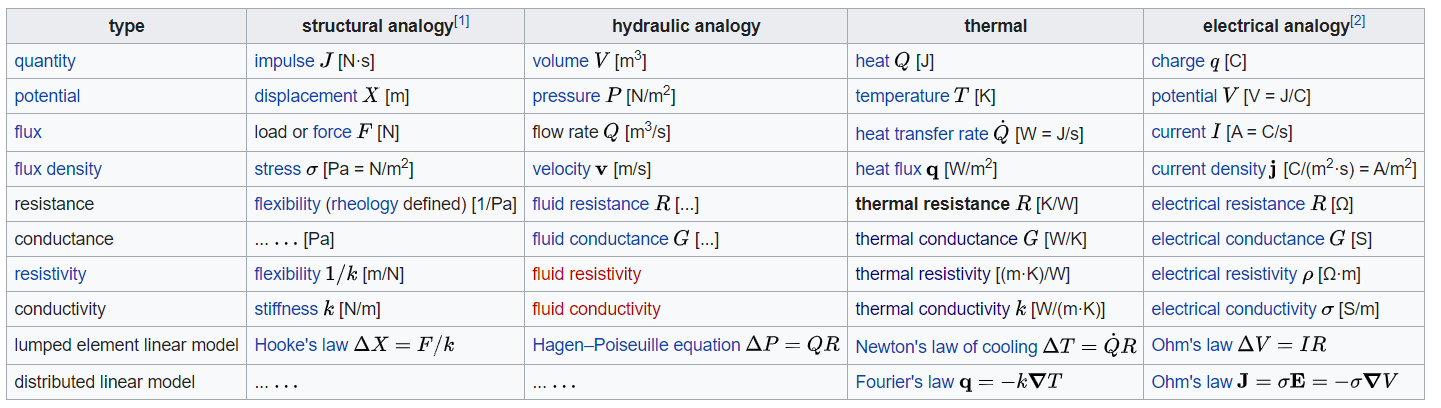
\includegraphics[width=1.0\columnwidth]{Pictures/Analogies.png}
	\caption[Short title]{Table of Analogies  \cite{AbsTR}}
	\label{fig:Analogies}
	\end{figure} 

The 2R-2C house model structure is implemented as described below. The schematic of an envelope house model has been shown in figure  \ref{fig:envelope2R2C} and the equivalent electrical 2R-2C network with components and topology is given in fig  \ref{fig:elec2R2C}.

\begin{figure}[H]
	\centering
	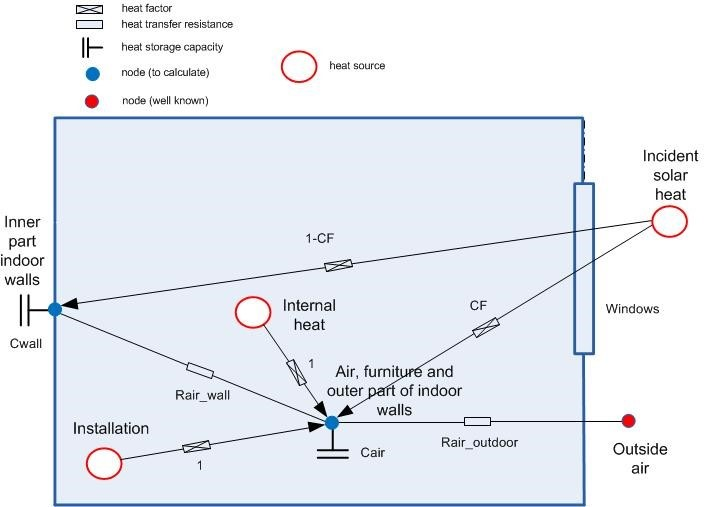
\includegraphics[width=1.0\columnwidth]{Pictures/envelopRC.jpg}
	\caption[Short title]{Schematic of envelope model}
	\label{fig:envelope2R2C}
	\end{figure} 

\begin{figure}[h!]
	\begin{center}
		\begin{circuitikz}
			\ctikzset{bipoles/thickness=3}
			\draw (0,0)
			to[V,v=$T_{outdoor}$] (0,4) % The voltage source
			to[R,R=$R_{air, out}$, -*] (4,4)
			node[color=red, circ, label={[red]above:$T_{air}$}]{}
			to[C=$C_{air}$] (4,0) % The heat capacity of the air
			to[short] (0,0);
			\draw(4,4)
			to[R,R=$R_{air, wall}$, -*] (8,4)
			node[color=red, circ, label={[red]above:$T_{wall}$}]{}
			to[C=$C_{wall}$] (8,0)
			to[short] (4,0)
			++ (-4,0);
		\end{circuitikz}
	    \caption{2R-2C house model.}
	    \label{fig:elec2R2C}
	\end{center}
\end{figure}

	
The model consists of two heat capacities C\textsubscript{air, indoor} and C\textsubscript{wall} and two resistances R\textsubscript{wall} and R\textsubscript{air, outdoor}. The incident solar energy is divided between C\textsubscript{wall} and C\textsubscript{air} through the convection factor CF. It is assumed that both internal heat (lighting, occupancy and electric devices) and supplied heat (installation) initially heat up the indoor air. In Fig. \ref{fig:envelope2R2C}, they are fully released at the T\textsubscript{air} node. 

 It is also assumed that furniture and the \textbf{surface part} of the walls have the same temperature as the air \textbf{and the wall mass is divided between the air and wall mass}. Thus, the heat capacity of the air node consists of the air heat capacity, furniture heat capacity and the heat capacity \textbf{of a part of the walls}. \textbf{Appendix A} presents the coefficients in the dwelling model. In the resistance R\textsubscript{air, outdoor} the influence of heat transmission through the outdoor walls and natural ventilation is considered. 
 
For the air and wall nodes the following power balances can be set up: 

\begin{equation}
C_{air}\frac{dT_{air}}{dt}=\frac{T_{outdoor}-T_{air}}{R_{air_{\_}outdoor}} + \frac{T_{wall}-T_{air}}{R_{air_{\_}wall}} + \dot{Q}_{inst} + \dot{Q}_{internal} + CF\cdot\dot{Q}_{solar}
\end{equation}

\begin{equation}
C_{wall}\frac{dT_{wall}}{dt}=\frac{T_{air}-T_{wall}}{R_{air_{\_}wall}} + (1-CF)\cdot\dot{Q}_{solar}
\end{equation}


 \begin{itemize}
      \item $CF$: convection factor (solar radiation): the convection factor is the part of the solar radiation that enters the room and is released directly convectively into the room.
      \item $\dot{Q}_{inst}$: delivered heat from heating system (radiator) [W].
      \item $\dot{Q}_{inernal}$: internal heat [W].
      \item $\dot{Q}_{solar}$: heat from solar irradiation [W].
      \item $T_{air}$: indoor air temperature $\degC$.
      \item $T_{outdoor}$: outdoor temperature $\degC$.
      \item $T_{wall}$: wall temperature $\degC$.
      \item $R_{air_{\_}wall}$: walls surface resistance [$\frac{K}{W}$].
      \item $R_{air_{\_}outdoor}$: outdoor surface resistance [$\frac{K}{W}$].
      \item $C_{air}$: air thermal capacity (heat capacity) [$\frac{J}{K}$]\cite{Thermalmass}.
      \item $C_{wall}$: wall thermal capacity (heat capacity) [$\frac{J}{K}$]\cite{Thermalmass}.
    \end{itemize}


Total heat transfer of solar irradiation through the glass windows: 
\begin{equation}
\dot{Q}_{solar}=g.\sum(A_{glass}.\dot{q}_{solar})
\end{equation}

\begin{itemize}
    \item $\dot{q}_{solar}$: solar radiation on the outdoor walls [$\frac{W}{m^2}$]. 
    \item g: g value of the glass (ZTA in dutch) [0..1]\cite{zontoetreding}
    \item A: glass surface [$m^2$].
\end{itemize}

%7.6.6.1.2 Ramen met niet-verstrooiende beglazing NTA8800
%https://help.dgmr.nl/bink9/zontoetredingsfactor-zta.html
%https://www.joostdevree.nl/shtmls/zta.shtml
%ISSO-Handboek Zonnestraling: 5.5.1 en 5.2


\newpage
